\chapter[Self-Resonant Micro-Helix at X-band]{Self-Resonant Micro-Helix for nano-Liter Volume Single-Crystals at X-band.\blfootnote{A significant portion of this chapter is from J.~W.~Sidabras, J.~Duan, M.~Winkler, T.~Happe,  R.~Hussein, A.~Zouni, D.~Suter, A.~Schnegg, W.~Lubitz, E.~J.~Reijerse, Sci. Adv., \textit{under review}.}}

For typical EPR experiments on proteins, a frozen solution of 0.1-1~mM concentration is prepared and placed in a microwave cavity. Standard sample volumes at X-band (nominally 9.5~GHz) are in the 200~$\mu$L range. However, frozen solution EPR experiments only allow the determination of the principal values of magnetic interactions at an active site, and thus provide only a limited view of the electronic structure. \cite{schweiger2001principles, goldfarb2018epr}

To resolve the full tensor magnetic interaction parameters, such as \textit{g}-, zero field, hyperfine-, and, for nuclei with $I>1/2$, quadrupole-tensors, single-crystal EPR experiments must be performed. In combination with X-ray crystallography, the magnetic-interaction tensors obtained with EPR experiments can be directly related to the protein geometry in order to help identify and better understand the catalytic mechanism of the enzyme. \cite{Bowman2016, NiFeRev2007} Despite its usefulness, single-crystal EPR is rarely applied to protein systems due to challenges in growing crystals of sufficient quality and volume for these experiments. Many protein crystals used in X-ray crystallography are of dimensions in the 50--300~$\mu$m range and, as such, are too small to be studied using commercial EPR instrumentation. Crystallization methods, such as macroseeding,\cite{macroseeding} have the potential to increase the volume of the crystals, but such techniques are difficult to implement. 

Currently, volume-limited crystals can only be studied using high-frequency EPR in a single-mode\cite{Hofbauer6623}, or, for continuous-wave experiments, Fabry-P\'{e}rot\cite{Klette94GHzPSI} resonators at W-band (94~GHz) or higher. Such high-frequency EPR spectrometers are not widely available and high-frequency conditions are usually unfavorable for advanced pulse experiments such as Electron Spin Echo Envelope Modulation (ESEEM) or Hyperfine Sub-level Correlation (HYSCORE) spectroscopies. \cite{pulseseq}

Unlike nuclear magnetic resonance (NMR), where all nuclei are excited and contribute to the NMR signal, hyperfine spectroscopy experiments, such as ESEEM, HYSCORE, and electron nuclear double resonance (ENDOR), probe only the nuclei that are magnetically coupled to the paramagnetic center. Extending these experiments to single crystals not only provides the magnitude of the hyperfine- and quadrupole-tensors of ligand nuclear spins that interact with the paramagnetic centers, but also the associated angles relative to the active site of an enzyme. Such interacting nuclei are either naturally abundant, such as $^1$H and $^{14}$N, or the catalytic cofactors can be enriched with nuclei such as $^2$H, $^{13}$C, $^{15}$N, and $^{57}$Fe, for further analysis of magnetic interaction tensors with respect to the first ligand-sphere. Furthermore, the same interaction tensors can be calculated from the molecular structure using quantum chemical calculations. \cite{NEESE2003125} These experimentally determined spectroscopic parameters can, therefore, be used to verify the adequacy of the level of theory which, in turn, gives confidence to the predicted electronic and geometric structure of the involved intermediates and transition-states in the whole catalytic cycle. The groundwork for understanding the inner workings of enzymes lies in collecting as much accurate spectroscopic information as possible, including other spectroscopic and structural methods (optical and vibrational spectroscopy, M{\"o}{\ss}bauer, X-ray spectroscopy, and diffraction). Every experiment contributes to the total picture and ultimately leads to a fundamental understanding of the catalytic mechanism of these enzymes.

To improve the sensitivity for studying single crystals using EPR on readily available spectrometers, typically at X-band, one must abandon the microwave cavity design and move to small-volume resonators based on lumped-circuits in the microwave frequency range. This allows the reduction of the sample volume by one order of magnitude, from 200~$\mu$L to 20~$\mu$L using a loop-gap resonator. \cite{hydehoff} Further reductions can be achieved by incorporating materials with a high dielectric constant in a standard resonator to reduce the active volume down to 1~$\mu$L. \cite{dielectricReson1, dielectricReson2} For protein single-crystals one must reduce the volume even further (less than 0.03~$\mu$L), which requires radical new approaches.

\begin{figure*}[htbp]
\centering
 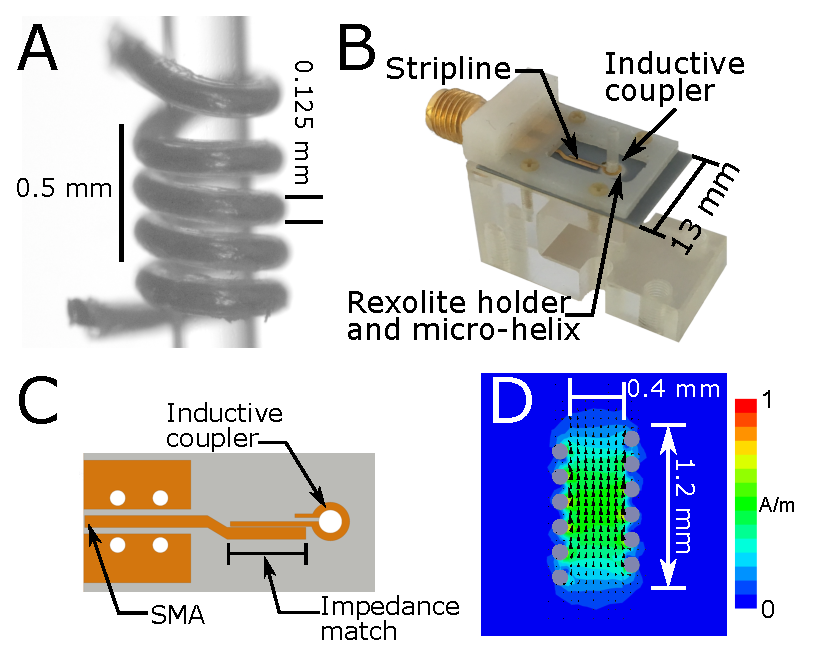
\includegraphics{Kapitel/Ch4-Images/01-MicroHelixHolder_Big2.eps}
 \caption[The self-resonant micro-helix.]{ The self-resonant micro-helix. A) A fabricated five-turn micro-helix wrapped around a 0.4~mm outer diameter capillary. During fabrication, the micro-helix is tightly wound around a 0.4~mm drill-bit and glued inside a Rexolite cylinder. The drill-bit is removed and the glue is allowed to dry for several days. The micro-helix assembly is placed in B) a coupling and support assembly, which includes a planar micro-coupler. C) The planar micro-coupler consists of a stripline impedance match to an inductive coupling loop. D) Finite-element modeling simulations of the microwave magnetic field, normalized to input power, at 9.5~GHz show an active region of good magnetic field homogeneity over a 0.8~mm height. The measured microwave magnetic field of 3.2 G/W$^{1/2}$ corresponds to a 20~ns $\pi$/2 pulse at approximately 20~mW. Dimensions of the micro-helix, where the self-resonance is determined by the capacitance formed between each turn and the inductance of the windings, are shown. The frequency can be tuned during fabrication by the number of turns, the pitch of the turns, or the inner diameter. The microwave characteristics of the fabricated micro-helix can be found in Table~\ref{table:chars}.}
 \label{fig:fabricated}
\end{figure*}

Herein, we combine the concept of a self-resonant micro-helix, shown in Fig.~\ref{fig:fabricated}A with that of a planar micro-coupler. The coupling structure on the printed-circuit board is a resonant structure which drives the self-resonant micro-helix placed in the center of the coupling loop\cite{coupling2016}, shown in Fig.~\ref{fig:fabricated}B. The micro-helix geometry offers significant advantages, in that, the microwave field homogeneity is strongly improved along with volume sensitivity for small samples, the microwave characteristics are optimal for pulse and continuous-wave experiments with need for very little microwave power, and the micro-helix assembly is easily matched and tuned over a variety of samples and temperatures.

\paragraph{Single-crystal EPR for metallo-enzyme research.}
For hydrogenases, specifically [NiFe]-hydrogenase, the single-crystal EPR strategy has been very successful. \cite{NiFe1996,NiFe2000, NiFe2003, NiFeRev2007} The active site of this enzyme harbors a [NiFe] binuclear cluster in which the iron carries two cyanide (CN$^-$) and one carbonmonoxide (CO) ligand. The metals are bridged by two cysteine thiols and the nickel center is further coordinated by two cysteine thiolate side groups. The paramagnetic states all originate from the nickel center, while the iron center remains Fe(II) during the catalytic cycle. \cite{lubitzhyd} The open-coordination site between the two metals can be occupied by an oxygen species leading to the inactive oxidized states or a hydride, which is the key intermediate in the catalytic cycle. \cite{NiFeRev2007} For all these species the $g$-tensor magnitude and orientation was determined and analyzed in terms of ligand-field theory and verified using quantum chemical calculations providing a fundamental insight into the electronic structure and the dependence on the first ligand-sphere. \cite{Ping2005, Gasteljp0573902, NiFeRev2007, LubitzNiFe2016} The [NiFe]-hydrogenase crystals in these studies were relatively large (2 $\times$ 0.5 $\times$ 0.5~mm$^3$) enabling measurements in standard X-band probe-heads with measuring time of 2-3 hours per angle, stepping over 180 degrees. However, even with the large crystal volume, ESEEM and HYSCORE experiments on [NiFe]-hydrogenase were only published in frozen solution with volumes of 50-200~$\mu$L and experimental times upwards of 2 hours for each experiment. \cite{NiFeRev2007} 

Similar experiments were anticipated for [FeFe]-hydrogenase which has a much higher activity and exhibits a different catalytic mechanism compared to [NiFe]-hydrogenase. Unfortunately, the crystals obtained from [FeFe]-hydrogenase are much smaller than those available from [NiFe]-hydrogenase with dimensions less than 0.3~mm. Frozen solution EPR on [FeFe]-hydrogenase has provided a lot of information on the binuclear active-site, such as, the discovery of a nitrogen in the dithiolate bridge (ADT-ligand). \cite{B905841A} However, the full $g$-tensor and the hyperfine-tensor, including angular information, of the active site are still elusive. Therefore, there is continuing interest in developing EPR instrumentation, specifically micro-resonators, at 9.5 and 35~GHz, X- and Q-band, respectively, optimized for metallo-enzyme research. Furthermore, other potentially interesting proteins (CODH\cite{C5CS00182J}, MMO\cite{Hoffman2014rev}, Rieske\cite{FERRARO2005175} and other Fe-S cluster containing proteins\cite{FeSClustersReview}) are rarely studied in single crystals, and doing so would contain a wealth of information on the electronic structure and enzymatic function. 

In this chapter, the design and implementation of a micro-helix is outlined. Experimental and simulated comparisons of the micro-helix geometry to commercially available and state-of-the-art resonator designs is presented. In order to further test the micro-helix geometry two experiments are performed on photosystem II tyrosine D radical: a 85~nl frozen solution and 0.3 $\times$ 0.18 $\times$ 0.18 mm$^3$ single crystal. These data demonstrate the utility of the micro-helix in studying protein single-crystals at volumes relevant for X-ray crystallography and provide a benchmark for future work.


\section{Methods}
All micro-helix and planar-coupling designs were modeled in the commercially available finite-element modeling program Ansys Electronics Desktop with HFSS (High Frequency Structure Simulator; v. 19.1) using driven mode. In driven mode, Ansys HFSS requires a coupling structure and mimics the output of a network analyzer. All designs are matched to 50~$\Omega$ with an S$_{11} < -35$~dB. Frequency and $Q$-values (-3~dB) are read directly from a simulated S$_{11}$-plot and $Q_0$-values are calculated by the known equation $Q=Q_0/(1+\beta$), where $\beta$ is the reflection coefficient at the frequency of resonance ($\beta=1$ for critically coupled). EPR signal intensity and resonator efficiency values (mT/W$^{1/2}$) were calculated using Ansys HFSS \cite{misrabook} and tabulated. EPR experimental comparisons were performed on an Elexsys E580 X-band bridge by Bruker Biospin. Four resonators are used for this comparison. The Bruker Biospin i) dielectric ER4118X-MD-5W1 (MD5W1) resonator and ii) LGR ER4118X-MS-3W1 (MS3; split-ring) resonators are used as comparisons with known commercial resonator geometries. Two $\Omega$-shaped 0.5~mm inner diameter PMR resonators are also tested. The first uses iii) Rogers 6010LM (RO6010LM printed-circuit board; Rogers Corp, Chandler, AZ, USA) substrate per Ref.~[5.\kern-0.4em\citenum{suter2015}] and one with (iv) sapphire substrate. The sapphire substrate was fabricated by Technical University Ilmenau (Ilmenau, Germany). Both PMR geometries have a 0.5~mm hole through the substrate. Resonator characteristics are found in Table~\ref{table:chars}. 

The continuous-wave EPR experiment measures the sample using a constant microwave power incident on the sample and slowly sweeping a quasi-static magnetic field through the resonance condition, $\nu =\gamma B_0$. Where $\nu$ is the operating frequency (nominally 9.5~GHz for X-band), $\gamma$ the the gyromagnetic ratio of the spin system ($\gamma = 2.8$~MHz/G for a free electron), and $B_0$ is the quasi-static magnetic field. The magnetic field is modulated, typically at 100~kHz, and collected using a phase-sensitive detector. \cite{weil2007electron} Continuous-wave is the standard EPR experiment. With modern digital signal processing and fast analog to digital converters, the continuous-wave experiment has recently been improved upon. The non-adiabatic rapid scan (NARS) \cite{KITTELL2011228, KITTELL201251, KITTELL201568, Hyde2013MDIFF, YU201558} and adiabatic rapid scan (RS) \cite{JOSHI200544,TSEITLIN200948, MITCHELL2012221, RScompare,MOSER2017} methods collect real and imaginary, pure-absorption and pure-dispersion, EPR spectra using fast quasi-static magnetic field or microwave frequency sweeps without the need for a phase-sensitive detector. Both rapid scan data can be pseudo-modulated to the conventional first-derivative EPR spectrum using a moving difference (MDIFF) pseudo-modulation. \cite{Hyde2013MDIFF} The non-adiabatic rapid scan (NARS) experiment uses a field sweep fast enough to overcome $1/f$ noise but remain in a thermal equilibrium, while adiabatic rapid scan sweeps the field fast enough to cause passage. The advantage of non-adiabatic rapid scan is the signal-to-noise improvement of collecting pure-absorption EPR spectra, while adiabatic rapid scan can further improve the continuous-wave and NARS experiment by changing the effective microwave magnetic field at the sample. This allows for an increase of microwave power, and thus, increase in EPR signal for saturable signals. \cite{JOSHI200544} While the non-adiabatic rapid scan method can be implemented on commercial bridges with no hardware changes, it does require some technical expertise. \cite{MOSER2017} However, to perform adiabatic rapid scan experiments on protein samples, custom current drivers are needed to increase the swept field amplitude. For simplicity, in this work, we have implemented only non-adiabatic rapid scan. Other experimental parameters are as stated in the manuscript.

The field-swept two-pulse electron spin-echo (ESE) experiment uses a ${\pi/2\!-\!\tau\!-\!\pi}$ pulse sequence ($\pi$ is 80~ns) that results in an echo $\tau$ seconds, herein $\tau$ is 300~ns, after the $\pi$ pulse. The field is stepped and a whole spectrum is acquired. This is the standard pulse sequence to collect an EPR spectrum. \cite{schweiger2001principles} 

Two EPR signal parameters were calculated in order to compare different resonant structures: i) unsaturable signal represents the EPR intensity at a given incident power, while ii) saturable signal represents the EPR intensity at a given microwave magnetic field that approaches the limit of saturation, i.e. the maximum achievable signal (P$_{1/2}$). For pulse experiments, the saturable signal is proportional to the EPR echo intensity in a two-pulse electron spin-echo (ESE) experiment. A 0.4~mm outer diameter and 0.3~mm inner diameter quartz capillary (QSIL GmbH, Ilmenau, Germany) with a 0.2~mm$^3$ ice sample ($\epsilon_r=3.17-i0.0035$, Ref.~[5.\kern-0.4em\citenum{icedielectric}] ) was used in the simulations. The signal-to-noise ratio for measured data is calculated by the ratio of the acquired signal mean to the standard deviation of the noise voltage, defined by
\begin{equation}
 \text{SNR}=\frac{S_{p\!-\!p}}{2\sigma_{noise}}
\end{equation}
where $S_{p\!-\!p}/2$ is the mean value of the peak-to-peak (or peak for absorption spectra) signal, and $\sigma_{noise}$ is the standard deviation of the noise. \cite{schroeder2000astronomical, oppenheim1999discrete} The standard deviation of the noise is calculated using 200 points in an off-resonance region.

The micro-helix is fabricated by hand winding 5 to 8 turns of 0.125~mm diameter silver wire with Polytetrafluoroethylene (PTFE) coating (0.0255~mm thickness, total 0.18~mm diameter; Science Products, GmbH, Hofheim, Germany) around a 0.4~mm drill bit and placed inside a Rexolite cylinder (0.8~mm inner diameter and 1.2~mm outer diameter) with a length of 10~mm. The drill bit is removed as the coil is affixed with super-glue by capillary action, waiting 1 minute, and blowing out the excess. The assembly is left to dry for several days. 

The coupling loop is designed in Ansys HFSS and prepared for fabrication in AutoDesk Inventor Professional 2019. The printed-circuit board designs are emailed to Streamline Circuit (Santa Clara, CA, USA) engineers and manufactured on a PTFE substrate. The printed-circuit board is connected to the bridge by a high-frequency SMA end launcher (AmphenolRF; 901-10510-1). Impedance matching is achieved by moving the micro-helix relative to the coupling loop until critically coupled on a network analyzer. Fine-tune matching is obtained with a slide-screw tuner at the bridge output. 

Comparison of resonator EPR characteristics were performed on an Elexsys E580 X-band bridge by Bruker Biospin. Four resonator geometries are used for this comparison. The Bruker Biospin i) dielectric ER4118X-MD-5W1 (MD5W1; sapphire $\epsilon_r$ of 11.5 parallel to C-axis and 9.3 perpendicular to C-axis) resonator and ii) Loop-gap resonator (LGR) ER4118X-MS-3W1 (MS3; split-ring) resonators are used as comparisons to known commercial resonator geometries. The dimensions of the MD5W1 and the MS3 can be found in Figs.~\ref{fig:geo}A and ~\ref{fig:geo}B, respectively. Additionally, two $\Omega$-shaped 0.5~mm ID planar micro-resonators (PMR) are also tested. \cite{Suter2005, Suter2008, NARKOWICZ201379, suter2015} The first PMR uses iii) Rogers 6010LM (RO6010LM; Rogers Corp, Chandler, AZ, USA) substrate and one with (iv) sapphire substrate. The sapphire substrate was fabricated by Technical University Ilmenau (Ilmenau, Germany). Both PMR geometries have a 0.5~mm hole through the substrate which allows for a capillary sample to be placed in the center of the resonator. The general geometry for the PMR is shown in Fig.~\ref{fig:geo}C.

\begin{figure}[htbp]
\centering
 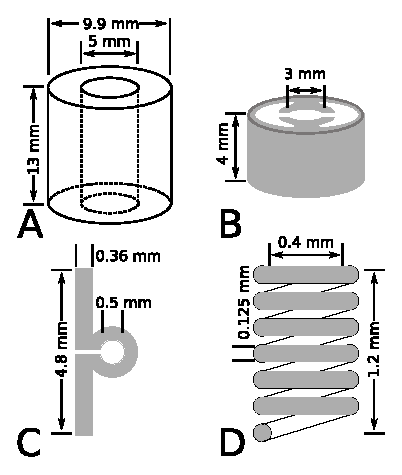
\includegraphics{Kapitel/Appendix/Images/S1-Geometries.eps}
 \caption[Geometries of resonators in this work.]{Dimensions and geometry of the four resonators compared in this paper. A) Bruker Biospin ER4118X-MD-5W1 (MD5W1) sapphire dielectric resonator, B) Bruker Biospin ER4118X-MS-3W1 (MS3) split-ring resonator, C) Planar Micro Resonator 0.5~mm inner loop diameter, and D) self-resonant micro-helix with a 0.4~mm inner diameter. Gray indicates metallic surfaces.}
 \label{fig:geo}
\end{figure}

The PMRs are fabricated by printing the micro-resonator geometry on a substrate using photo-lithographic techniques. \cite{Suter2005, Suter2008, suter2015} The planar micro-resonators show significant improvement in absolute spin sensitivity compared to the best commercial probe-heads available. \cite{ ReijerseSavitsky2017} PMRs can be produced relatively cheaply using semiconductor etching techniques and laser scribing, and configured for many frequencies with inner diameter sample sizes of 20-1000 $\mu$m. Furthermore, these structures offer excellent filling factors, high resonator efficiencies, and minimal power dissipation. It was recently demonstrated that a planar micro-resonators with Rogers RO6010LM substrate and a 500~$\mu$m sample diameter can be successfully employed for the study of crystals of inorganic metal complexes as well as [NiFe]-hydrogenase (0.35 $\times$ 0.2 $\times$ 0.2~mm$^3$) at 14~GHz, equipped with a specially designed cryogenic receiver at a temperature of 12~K. \cite{NARKOWICZ201379} Yet, such designs require a modified bridge to accommodate the cryogenic amplifier setup.

\begin{figure}[htbp]
\centering
 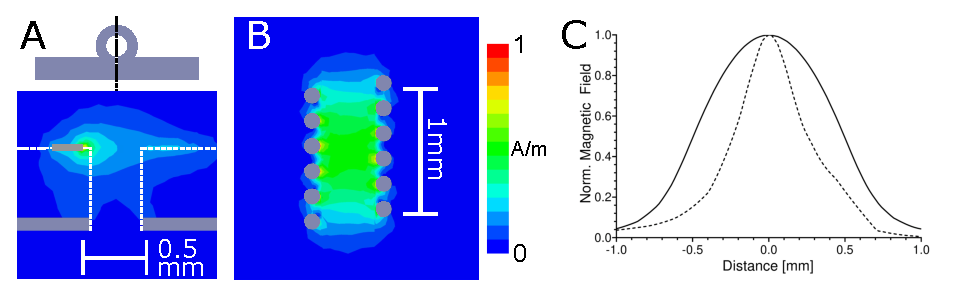
\includegraphics[width=\textwidth]{Kapitel/Ch4-Images/02-PMRCompare_OnAxis.eps}
 \caption[Ansys HFSS magnetic field simulation: PMR and micro-helix.]{Ansys HFSS finite-element modeling simulation of the microwave magnetic fields of a A) $\Omega$-shaped planar micro-resonator on sapphire substrate (dashed white lines; cut-plane shown on inset) with a 0.5~mm sample diameter over a ground plane and a B) 5.5 turn micro-helix with a 0.4~mm inner diameter. Normalized microwave magnetic field, for both resonators at the same power, is shown on the right. C) Normalized microwave magnetic field on axis of a $\Omega$-shaped planar micro-resonators on sapphire substrate with a 0.5~mm sample diameter over a ground plane (dashed lines) and a 6.5 turn micro-helix with a 0.4~mm inner diameter (solid).}
 \label{fig:HFSS}
\end{figure}

Due to their planar geometry, PMR designs are limited in their $Q$-value (50-180) and suffer from a strong inhomogeneity of the microwave magnetic field, illustrated in Fig.~\ref{fig:HFSS}A compared to the microwave magnetic field of the self-resonant micro-helix, Fig.~\ref{fig:HFSS}B. The microwave magnetic field comparison on axis can be found in Fig.~\ref{fig:HFSS}C. Improvement of the $Q$-value of the PMR geometry are reported here. By changing the substrate from Rogers RO6010LM substrate to single-crystal sapphire the $Q$-value increases by a factor of 3. The reduction of the $Q$-value using the Rogers RO6010LM substrate is partially due to surface roughness, and not just the loss tangent of the material. Because of these challenges, the PMRs have room for improvement and exploration of different geometries have led to the self-resonant micro-helix. Therefore, in this work, we compare the self-resonant micro-helix, general geometry shown in Fig.~\ref{fig:geo}D, to the planar micro-resonators.

Simulations, from the commercially available finite-element modeling program Ansys Electronics Desktop with HFSS (High Frequency Structure Simulator; v. 19.1), network analyzer, and experimental measurements of resonator characteristics are tabulated in Table~\ref{table:chars} and in Table~\ref{table:signal}. Simulations are performed assuming a fixed sample volume of 0.1~mm diameter by 0.1~mm height cylindrical sample. The simulated sample allows for absolute sensitivity comparisons amongst the resonator designs. Experimentally, a minuscule amount of lithium phthalocyanine (LiPC)\cite{Liu5438} is embedded in Crytoseal (or similar) wax and is used as a point sample. The LiPC sample produces a very sharp line width (less than 0.05~mT) in the presence of oxygen (narrower without oxygen present), saturates at large values of ${\mathbf B}_{1r}$, and one needs very little sample volume to observe the signal. Therefore the use of LiPC allows for a fair comparison between all resonators by using the same sample throughout the experiments. The term ``minuscule'' is defined as enough sample to observe a signal in the Bruker MD5W1 without causing line broadening in the micro-helix geometry. Such line broadening is due to a radiation dampening-like behavior caused by the very-large filling factor $\eta$.

Bench tests of resonator characteristics, such as the frequency measurements, $Q_0$-value, and sample frequency shifts, were performed on an Agilent 8722ES (now Keysight Technologies; Santa Rosa, CA, USA) vector network analyzer.

The photosystem II complex sample from spinach was prepared by following the BBY method and placed in a 0.4~mm outer diameter capillary with a 0.3~mm inner diameter. \cite{BBY1981} The tyrosine D (Y$_D^\bullet$) radical is generated by ambient light at room temperature for a few minutes and then rapidly frozen in liquid nitrogen. The Y$_D^\bullet$ radical is well-suited as a biological test sample since it has been extensively studied and the g- and hyperfine tensors are known. \cite{Hofbauer6623} Using UV-VIS spectroscopy, the number of chlorophyll molecules in the sample can be determined and, taking into account that there are approximately 250 chlorophyll molecules per photosystem II complex in spinach, the approximate amount of enzyme can be calculated. Each photosystem II complex contains one Y$_D^\bullet$ radical. For the sample prepared in this work, 7.9~$\mu$M/mL of chlorophyll molecules were measured, resulting in approximately 1.6$\times10^{12}$ Y$_D^\bullet$ radicals in the 85~nl that fill the micro-helix. 

Additionally, photosystem II core complex, extracted and purified from the thermophilic cyanobacterium {\em Thermosynechococcus elongatus}, has been crystallized to reach a crystal size of 0.3 $\times$ 0.18 $\times$ 0.18 mm$^3$, using the method of Athina Zouni and colleagues. \cite{KERN2005147} The crystals were gradually transferred to a cryogenic protection buffer (100~mM MES, pH 6.5, 5~mM CaCl$_2$ , 30\% (w/w) glycerol, 16\% PEG2000). The photosystem II core complex forms a dimer and the crystal has a unit cell space group symmetry P${2_1\,2_1\,2_1}$ which generates two asymmetric units per unit cell (PDB ID: 1W5C). From this one can calculate that there are approximately 8.9$\times10^{12}$ Y$_D^\bullet$ radicals in the test crystal. The active center and the Y$_D^\bullet$ of a cyanobacterium is equivalent to that of the photosystem II from spinach. 

\section{Theory and Design}
We focus on the development of resonant structures to increase EPR absolute spin sensitivity at X-band without the use of super-conducting materials, which require temperatures that are sub-optimal for metallo-enzyme research and exhibit $Q$-values too large for pulse experiment, or commercial bridge modifications, which require technical expertise not commonly available in EPR laboratories. We start with the well-established EPR signal analysis by Feher,\cite{FeherSignal} which states that the continuous-wave EPR signals for a critically-coupled resonator on a reflection bridge is proportional to
\begin{equation}
 S \propto \chi \eta Q P^{1/2},\label{eq:feher}
\end{equation}
where $\chi$ is the magnetic susceptibility, $Q$ is the $Q$-value of the cavity, $P$ is the incident power, and $\eta$ is the filling factor. The $Q$-value is defined as the ratio of the stored energy in the resonator to the power loss in the sample and resonator. \cite{ginzton1957microwave} While, the filling factor is defined as the ratio of the circularly polarized microwave magnetic field stored energy perpendicular to the static magnetic field that gives rise to EPR transitions and the complete magnetic field stored energy in the geometry,
\begin{equation}
 \eta = \frac{\int {\mathbf B}_{1r} \cdot {\mathbf B}_{1r}^* dV_s}{\int {\mathbf B}_1 \cdot {\mathbf B}_1^* dV},
\end{equation}
where ${\textbf B}_1$ is the microwave magnetic field in all space ($V$) and ${\textbf B}_{1r}$ is one component of the clockwise (or counter clockwise) rotational component of the linear ${\textbf B}_1$ field perpendicular to the static magnetic field in the sample volume ($V_s$). \cite{FeherSignal, misrabook}

From Eqn.~\ref{eq:feher}, we can derive a metric that encompasses the filling factor $\eta$ and the Q-value, called the resonator efficiency. \cite{hydehoff} The resonator efficiency (or, conversion factor) is defined as 
\begin{equation}
 \Lambda = \frac{\left|{\mathbf B}_{1r}\right|}{\sqrt{P_l}} \qquad [\text{mT/W}^{1/2}],
\end{equation}
where $P_l$ is the power loss in the system, including sample. However, $\Lambda$ assumes that the microwave magnetic field is uniform and does not take into account non-uniformity of the field over the sample. Experimentally, the microwave magnetic field is distributed throughout the sample and the average of $\Lambda$ is measured. We can define the resonator efficiency average as
\begin{equation}
 \Lambda_{ave} = \frac{\int |{\mathbf B}_{1r}| dV_s}{\sqrt{P_l} V_s} \qquad [\text{mT/W}^{1/2}].
\end{equation}
The resonator efficiency average is proportional to the signal and, for a fixed volume, is proportional to the absolute spin sensitivity. 

Cavity resonators, such as the Bruker Super High-Q probe head, are not sufficiently sensitive for extremely small samples since the very small filling factor $\eta$ is not compensated by the high Q-value, resulting in a poor EPR signal. \cite{ReijerseSavitsky2017} Therefore, one way to maximize $\Lambda_{ave}$ is to reduce the size of the resonant structure relative to the sample volume, increasing the filling factor. The challenge arises due to potentially increasing the losses in the system, degrading the Q-value, more than the increase in the filling factor. Two common methods to reduce the size of a resonant geometry is to either use dielectric resonators (DR) to reduce the wavelength and, consequently, the size of the resonator or loop-gap resonators (LGR) to reduce the cut-off frequency of a waveguide by introducing protrusions to create regions of inductive loops and capacitive gaps. (Dielectric resonator and LGR geometries with commercially available dimensions are illustrated Fig.~S1 and the microwave characteristics are tabulated in Table~\ref{table:chars}.) However, in order to study sample volumes less than 0.03~$\mu$L, further resonator reduction strategies are needed.

Limitations to minimizing LGR geometries stem from an increase in Ohmic losses due to a reduction in the gap spacing to maintain a constant resonant frequency as the sample-loop radius is reduced. In practice, this has put a limit on the $\Lambda_{ave}$ obtainable to less than 1~mT/W$^{1/2}$ for X-band. Further EPR signal improvement is possible using dielectric resonators by increasing the dielectric permittivity, and dielectric resonators with permittivity up to 80 have been used for continuous-wave EPR experiments on crystals of porous materials and polymers. \cite{dielectricReson1, dielectricReson2} However, such resonators exhibit Q-values over 2500 that make pulse experiments problematic. \cite{Friedlaender2015} 

Several other approaches have been followed to develop application-specific resonators for micro-samples: microstrip resonators (MR)\cite{Microstrip2009, GhirriMicroStrip}, ultra-miniature micro-resonators (UMR, 2-150 $\mu$m)\cite{AharonBlankUltra2013}, surface loop-gap micro-resonators (LGMR, 50-150 $\mu$m)\cite{AharonSurface2010}, very high-permittivity dielectric resonators \cite{walsh86, GOLOVINA200852}, and planar micro-resonators. \cite{Suter2005, Suter2008, suter2015} All of which significantly reduce the size of the resonator, but have challenges that limit the usefulness for single-crystal experiments. Herein, we introduce a new type of resonator based on a self-resonant micro-helix which is particularly useful for protein single-crystal experiments at X-band and can be used as a drop-in replacement on a standard commercial system. The self-resonant micro-helix geometry, illustrated in Fig.~\ref{fig:fabricated}, solves these challenges by providing good magnetic field homogeneity, a high efficiency parameter, an optimum $Q$-value for both pulse and continuous-wave EPR experiments, straight-forward impedance matching, and ease of sample placement. 

Helical resonators were first introduced to EPR in the early-1960s as a method to increase the microwave magnetic field at the sample. Resonant helical geometries were affixed to one end of a shorted waveguide creating a slow-wave structure. \cite{Webb1962, Helix1967} Coupling was achieved by direct connection to a coaxial line with a capacitive matching network or by microwave incident on the helical structure from a waveguide. The sample was placed within the helix and showed reasonable sensitivity increase and larger microwave magnetic field due to higher filling factors compared to typical cavities. \cite{Nolle1966} Broadband slow-wave helical resonators were employed for multi-frequency experiments, where a non-resonant structure, having a $Q$-value close to unity, could be matched with a slide-screw tuner over an octave bandwidth. \cite{nonresonant1986} However, over time, they were replaced by loop-gap resonators which achieved higher concentration sensitivity for limited samples.\cite{froncisz1982loop}

Recently, micro-coils have gained popularity in NMR for nano-liter samples \cite{Olson1967, SUBRAMANIAN1998227, cr980140f,Kentgens2008,Raluca2011,Jones2012} and for microfluidics. \cite{Mompean2018} However, three characteristics differentiate our micro-helix configuration from those described in the EPR \cite{Webb1962, Helix1967, oldmicro} and NMR literature\cite{WEBB2005892}: i) the helix is self-resonant, meaning that the self-inductance of $n$-turns ($L_{tot}$) and self-capacitance between the loops ($C_{tot}$) resonate at a frequency determined by $\omega^2 L_{tot}C_{tot}=1$, where $\omega$ is the resonant frequency in radians/s. Since the geometry is self-resonant, no additional capacitors are needed. A self-resonant micro-helix has lower Ohmic loss, which provides a higher $Q$-value than is typically feasible with micro-coil geometries in NMR, where, with an NMR micro-coil, a typical $Q$-value is around 30. \cite{WEBB2005892} With a self-resonant micro-helix, the volume to surface ratio is maximized and a $Q$-value of 300 is achievable. ii) The helix length is much smaller than the wavelength (31.6~mm at 9.5~GHz), which increases the uniformity and the inner diameter is 0.4~mm at X-band, which increases the resonator efficiency. With this geometry, the micro-helix is not a slow-wave structure but an inductor at self-resonance. The microwave magnetic field profile is shown in Fig.~\ref{fig:fabricated}D. iii) Finally, the helix is coupled to an inductive coupling loop on a printed-circuit board by mutual inductance, which can be designed to minimize noise and further increase the EPR signal-to-noise ratio. \cite{coupling2016} Additionally, mutual inductance coupling does not require a balun or capacitive matching networks, simplifying coupling methods.

\paragraph{Qualitative Sensitivity Comparison of the X-band micro-helix to High-frequency single-mode resonators.}
Simulations were performed in commercial finite-element modeling software, Ansys Electronics Desktop with HFSS (High Frequency Structure Simulator; v. 19.1), comparing a cylindrical TE$_{011}$ cavity at W-band to the micro-helix geometry using a 85~nl frozen solution sample. Assuming no g-anisotropy, the W-band TE$_{011}$ exhibits a factor of approximately 3 in improved EPR signal intensity compared to the micro-helix geometry at X-band. However, for example, the g-anisotropy at W-band spreads the tyrosine D radical in photosystem II spectrum by a factor of 2 (see Fig.~2 in Ref.~[5.\kern-0.4em\citenum{Hofbauer6623}]); for some systems, the g-anisotropy may be more severe. Therefore, the micro-helix EPR sensitivity at X-band is comparable to a standard W-band system with a cylindrical TE$_{011}$ cavity. 

As the frequency becomes even higher, the resonator efficiency decreases due to losses on the surface of the resonator. For example, the Bruker 263~GHz single-mode resonator has a reported $\Lambda_{ave}$-value of 0.7 mT/W$^{1/2}$. \cite{bruker263} This is approximately half of the cylindrical TE$_{011}$ cavity at W-band. The lower $\Lambda_{ave}$ leads to only a factor of five in EPR signal improvement compared to the micro-helix at X-band. However, g-anisotropy becomes more severe as the operating frequency increases.

Therefore, the micro-helix geometry opens up the possibility to perform multi\-/frequency EPR on the same sample from X-band to 263~GHz. Using a 0.4~mm outer diameter capillary, a sample can be placed in the micro-helix at X-band and the same sample can then be inserted into a W-band (94~GHz) or 263~GHz cavity. This ability allows for complimentary techniques to be used for disentangling the angle dependencies of hyperfine-tensor interactions.

\section{Results and Discussion}
\subsection{EPR Characteristics Comparison of Resonators.}
Good agreement is shown in Table~\ref{table:chars} and in Table~\ref{table:signal}. The lower measured $Q$-value of the self-resonant micro-helix is due to losses associated with the Polytetrafluoroethylene (PTFE) substrate of the printed-circuit board and losses in the super-glue adhesive. Further work to minimize these losses is underway.

\begin{table}[htbp]
\centering
\caption[Resonator characteristics calculated and measured.]{Resonator characteristics calculated and measured. Calculations use fixed volume sample of dimension  0.1~mm diameter by 0.1~mm height cylindrical sample while measurements use a minuscule amount of lithium phthalocyanine (LiPC) in a 0.4~mm outer diameter and 0.3~mm inner diameter capillary tube. The P$_{1/2}$-values are measured from the power saturation curve and are related to the calculated $\Lambda_{ave}^2$. The $\Lambda_{ave}$ measurements were made by a 2\% w/w BDPA ($\alpha$,$\gamma$-Bisdiphenylene-$\beta$-phenylallyl; Sigma-Aldrich Chemicals; CAS number 35585-94-5) in polystyrene with dimensions of 0.55$\times$0.18$\times$0.08~mm$^3$.}
\label{table:chars}
\begin{tabular}{l|c|c|c|c|c}
\multicolumn{1}{l}{} & DR & LGR & \multicolumn{2}{c|}{PMR} &  \\
\multicolumn{1}{c||}{Geometry} & MD5W1 & MS3 & 6010LM & Sapphire & Micro-Helix \\ \hline \hline
\multicolumn{1}{l||}{Freq. Calc.} & \multicolumn{1}{c|}{9.67} & \multicolumn{1}{c|}{9.67} & \multicolumn{1}{c|}{9.87} & \multicolumn{1}{c|}{9.87} & 9.78 \\ \hline 
\multicolumn{1}{l||}{Freq. Meas.} & \multicolumn{1}{c|}{9.69} & \multicolumn{1}{c|}{9.69} & \multicolumn{1}{c|}{9.58} & \multicolumn{1}{c|}{9.58} & 9.73 \\ \hline 
\multicolumn{1}{l||}{$Q_0$-value Calc.} & \multicolumn{1}{c|}{8860} & \multicolumn{1}{c|}{870} & \multicolumn{1}{c|}{90} & \multicolumn{1}{c|}{190} & 360 \\ \hline 
\multicolumn{1}{l||}{$Q_0$-value Meas.} & \multicolumn{1}{c|}{6650} & \multicolumn{1}{c|}{600} & \multicolumn{1}{c|}{61} & \multicolumn{1}{c|}{181} & 220 \\ \hline
\multicolumn{1}{l||}{$\Lambda$ Calc. {[}mT/W$^{1/2}${]}} & \multicolumn{1}{c|}{0.60} & \multicolumn{1}{c|}{0.68} & \multicolumn{1}{c|}{1.9} & \multicolumn{1}{c|}{2.9} & 4.1 \\ \hline 
\multicolumn{1}{l||}{$\Lambda_{ave}$ Calc. {[}mT/W$^{1/2}${]}} & \multicolumn{1}{c|}{0.60} & \multicolumn{1}{c|}{0.68} & \multicolumn{1}{c|}{1.5} & \multicolumn{1}{c|}{2.6} & 4.0 \\ \hline 
\multicolumn{1}{l||}{P$_{1/2}$ Meas. {[}mW{]}} & \multicolumn{1}{c|}{19.2} & \multicolumn{1}{c|}{18.4} & \multicolumn{1}{c|}{17.3} & \multicolumn{1}{c|}{1.8} & 0.8 \\ \hline 
\multicolumn{1}{l||}{$\Lambda_{ave}$ Meas. {[}mT/W$^{1/2}${]}} & \multicolumn{1}{c|}{–} & \multicolumn{1}{c|}{–} & \multicolumn{1}{c|}{–} & \multicolumn{1}{c|}{2.2} & 3.2
\end{tabular}
\end{table}


\paragraph*{Comparison of a Planar micro-Resonator and micro-Helix}
In Chapter 5, the planar micro-resonator (PMR) \cite{Suter2005,Suter2008,suter2015} and micro-Helix geometries are thoroughly introduced. In this section we will construct an eigenmode solution of both the PMR and micro-helix to compare how the signal and resonator efficiency $\Lambda_{ave}$ scale with a lossy aqueous sample ($\epsilon_r = 63 - i26.46$ from Ref.~[5.\kern-0.4em\citenum{EllisonWater2017}]) and relatively-lossless ice sample ($\epsilon_r=3.17-i0.0035$ from Ref.~[5.\kern-0.4em\citenum{icedielectric}]). 

The files can be found at https://github.com/jsidabras/HFSSTutorial and the Ansys \textit{aedt} file has 4 projects to be solved. The projects created use local variables for performing parametric sweeps. For instance, the sample radius on both geometries can be varied and this parameter will be used in this comparison. Mesh operations have been added on the quartz capillary tube and on the surface of the main resonator geometry to reduce numerical fluctuations and obtain a field profile void of discontinuities. An eigenmode solution is used for simplicity. 

\begin{figure}[ht]
 \centering
 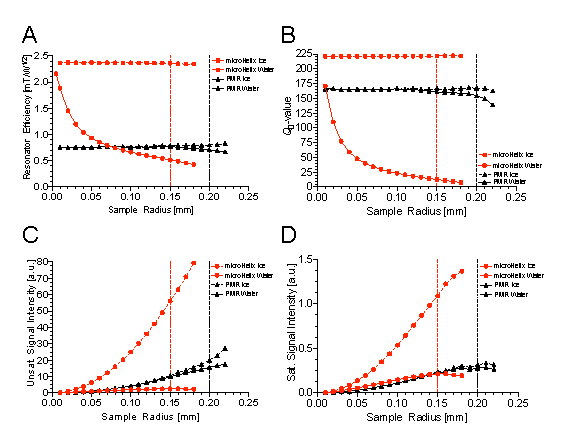
\includegraphics[width=\textwidth]{Kapitel/Ch2-Images/Ch2-SweepOutput.eps}
 \caption[EPR characteristics as the sample radius is swept.]{EPR characteristics for the PMR with sapphire substrate (black; $\blacktriangle$) and the 0.4~mm micro-helix (red; $\CIRCLE$) with a water (solid) and ice (dashed) sample. Shown are the EPR characteristics as the sample radius is swept for the A) resonator efficiency $\Lambda$, B) $Q_0$-value, C) unsaturated EPR signal, and D) saturable EPR signal. The dashed-dot lines indicate the largest practical capillary inner radius for the helix (red) and PMR (black).}
 \label{fig:SweptData}
\end{figure}

Shown in Fig.~\ref{fig:SweptData} are the simulated EPR characteristics for the micro-helix (red; $\CIRCLE$) and planar micro-resonator (black; $\blacktriangle$) geometries. The ice sample is shown as a dashed line, while the aqueous sample is shown as a solid line. The sample radius is swept and a quartz sample holder with a wall thickness of 0.025~mm is used. The dashed-dot line indicates the largest commercially available practical capillary inner radius for the helix (red) and PMR (black). In this study, we focus on a ``concentration sensitivity'' comparison. By comparing ``concentration sensitivity'' we focus on the resonator performance assuming a varying sample volume at a fixed concentration.

\begin{figure}[ht]
 \centering
 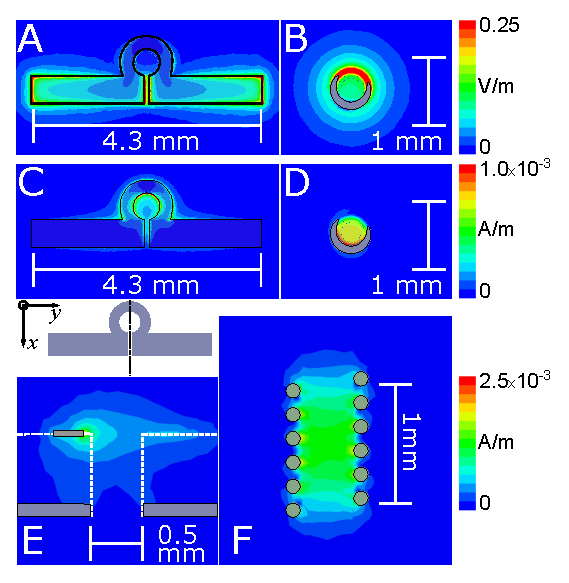
\includegraphics[width=0.9\textwidth]{Kapitel/Ch2-Images/Ch2-AnsysFields.eps}
 \caption[Simulated field distribution for Helix and PMR.]{Simulated field distribution for the magnitude of the electric field for the A) planar micro-resonator and B) micro-helix and the magnitude of $\mathbf{H_{1r}}$ with $\mathbf{H}_0$ in the $y$-direction for the C) planar micro-resonator and D) micro-helix in the $x$-$y$-plane. And the magnitude of $\mathbf{H_{1r}}$ with $\mathbf{H}_0$ in the $y$-direction for the E) planar micro-resonator and F) micro-helix in the $x$-$z$-plane. }
 \label{ch2-fig:FieldData}
\end{figure}

For the PMR (black; $\blacktriangle$), little change in both the average resonator efficiency $\Lambda_{ave}$ and $Q_0$-value is exhibited as the sample radius is increased, Figs.~\ref{fig:SweptData}A and \ref{fig:SweptData}B, respectively. From the simulations we can see that the electric field, which gives rise to losses, is well contained in the planar micro-resonator geometry away from the sample loop. Shown in Fig.~\ref{ch2-fig:FieldData}A is a plot of the magnitude of the electric field. A potential is formed across the PMR gap and a gradient of charge is formed in the loop which goes to zero opposite of the gap. This is similar to the electric field profile of a one-loop--one-gap loop-gap resonator.  

In the PMR, the value of $\Lambda_{ave}$ is approximately one third of the micro-Helix (red $\CIRCLE$; in Fig.~\ref{fig:SweptData}A). The reduction in $\Lambda_{ave}$ is due to a significant portion of the magnetic field stored energy being located outside of the sample volume in the PMR geometry and significant inhomogeneity of the magnetic field along the axis. This is illustrated in Fig.~\ref{ch2-fig:FieldData}C where the magnitude of $\mathbf{H_{1r}}$ with $\mathbf{H}_0$ in the $x$-direction is plotted. The quantity $\mathbf{H_{1r}}$ is the magnetic field that gives rise to the EPR signal and a significant portion of this magnetic field lies outside of the sample region. This is also true along the axis, shown in Fig.~\ref{ch2-fig:FieldData}E, where a large gradient of $\mathbf{H_{1r}}$ is present. 

With the micro-helix geometry, the $\mathbf{H_{1r}}$ is concentrated in the center and very little magnetic field is found outside of the sample volume, shown in Fig.~\ref{ch2-fig:FieldData}D. Additionally, the $\mathbf{H_{1r}}$ field profile along the axis is more homogeneous compared to the PMR, shown in  Fig.~\ref{ch2-fig:FieldData}F. The homogeneous magnetic field in the micro-helix leads to a higher filling factor $\eta$ and, ultimately, a higher average resonator efficiency $\Lambda_{ave}$, as shown in Fig.~\ref{fig:SweptData}A.

As anticipated from Eqn.~\ref{ch2-eq:su}, relatively lossless samples will display EPR unsaturable signal growth that is proportional to the magnetic field squared within the sample volume, shown in Fig.~\ref{fig:SweptData}C as a dashed line for the micro-helix (red; $\CIRCLE$) and PMR (black; $\blacktriangle$). With such samples, the EPR signal expected by using the micro-helix is significantly enhanced compared to the PMR. In contrast, the saturable sample defined by  Eqn.~\ref{ch2-eq:ss} has a maximum due to the interplay of the power loss $P_l$ and the magnetic field in the sample. Since the micro-helix exhibits an azimuthal component of the electric field that penetrates into the sample, shown in Fig~\ref{ch2-fig:FieldData}B, lossy aqueous samples are problematic in this geometry. Likewise, the  resonator efficiency $\Lambda_{ave}$ and $Q_0$-value are significantly reduced as the diameter of the aqueous sample increases, shown in Fig.~\ref{fig:SweptData}A and \ref{fig:SweptData}A, respectively.

Aqueous sample simulations show that the PMR losses do not increase with the size of the sample and little changes of the unsaturable and saturable signal are illustrated, shown as a solid black line in Figs.~\ref{fig:SweptData}C and \ref{fig:SweptData}D. Compared to the micro-helix geometry with lossy aqueous samples, the PMR performs 5 times better for experiments at the same microwave power (unsaturable signal) and 50\% better for the experiments at same microwave field (saturable signal). This means the PMR geometry may be advantageous for room temperature samples and further improvement to the PMR to increase the filling factor $\eta$ is underway. 

\begin{figure}[ht]
 \centering
 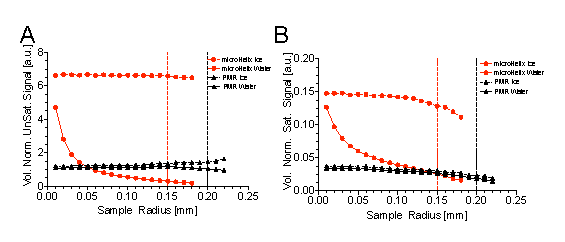
\includegraphics[width=\textwidth]{Kapitel/Ch2-Images/Ch2-AbsSweepOutput.eps}
 \caption[Volume normalized swept EPR signal optimization.]{Volume normalized Swept EPR signal for the PMR with sapphire substrate (black; $\blacktriangle$) and the 0.4~mm micro-helix (red; $\CIRCLE$) with a water (solid) and ice (dashed) sample. Shown are the data fro the A) unsaturated EPR signal and B) saturable EPR signal normalized to sample volume. The active region of the micro-helix and planar micro-resonator is assumed to be 1.2~mm and 1.1~mm, respectively. The dashed-dot line indicates the largest practical capillary inner radius for the helix (red) and PMR (black).}
 \label{fig:AbsSweptData}
\end{figure}

This example assumed the sample tube is completely filled and extends beyond the active region. It is noted that, the active length of the two resonators is different and the data plotted in Fig.~\ref{fig:SweptData} can be normalized to the active volume and a comparison of the ``absolute sensitivity'' can be performed. Based on the magnetic field profile of  Figs.~\ref{ch2-fig:FieldData}E and \ref{ch2-fig:FieldData}F, the active region of the micro-helix and planar micro-resonator is assumed to be 1.2~mm and 1.1~mm, respectively, and a volume normalized signal is plotted in Fig.~\ref{fig:AbsSweptData}. Comparing the resonators at a equivalent sample volume is the focus of Chapter~5 for single-crystal EPR of with sample volumes smaller than 27~nl. At a fixed sample volume, the losses in the micro-helix associated with the aqueous sample still significantly affect the performance of the resonator, plotted in Figs.~\ref{fig:AbsSweptData}A and \ref{fig:AbsSweptData}B as a solid line for the micro-helix (red; $\CIRCLE$). However, compared to the PMR (black; $\blacktriangle$) there exists some sample volumes where the micro-helix yields a higher EPR signal. Finally, at a fixed sample volume and a relatively lossless sample, the micro-helix significantly outperforms the PMR geometry, plotted in Figs.~\ref{fig:AbsSweptData}A and \ref{fig:AbsSweptData}B as a dashed lines.

This simple optimization sweep teaches about differences in such simple geometries and leads to intuition for further performance improvements. For instance, there is room for improvement for small volume aqueous samples. Such improvements would focus on reducing the electric field in the sample while maintaining good magnetic field homogeneity. 


\paragraph{Power Saturation and $\Lambda_{ave}$ Measurements}
Power saturation experiments were performed using the LiPC sample and plotted in Fig.~\ref{fig:lipcpwrsat}. From the power saturation data, an unsaturable signal, saturable signal, and P$_{1/2}$-value measurement can be ascertained. The unsaturable signal is measured at constant microwave power (0.01~mW), while the saturable signal is measured at the power where the EPR signal amplitude is maximum (P$_{1/2}$-value; indicated by $\Diamond$). At the P$_{1/2}$-value, the B$_{1r}$ over the sample is identical in each of the resonators. For the power saturation experiments used in this work the microwave power was stepped in 3~dB increments from 200~mW to 0.2~$\mu$W (0-60~dB). Each scan was 30~s over 1~mT with 4096 pts, receiver gain of 60~dB and 100~kHz field modulation at 0.1~mT in all resonators. The over-modulation of the LiPC sample was used to increase the sensitivity in the Bruker commercial resonators while increasing the intrinsic line width (line-height--line-width compromise, discussed in Ref.~[5.\kern-0.4em\citenum{eaton2010quantitative}]). 

\begin{figure}[htbp]
\centering
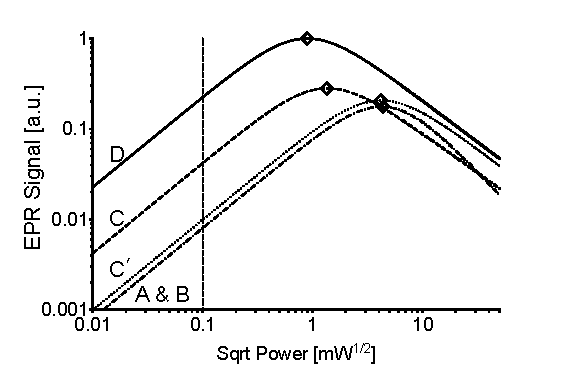
\includegraphics{Kapitel/Appendix/Images/S4-LiPCPowerSat.eps}
\caption[Power saturation data of LiPC comparing resonators.]{Power saturation data of LiPC showing the A) Bruker MD5 (dash-dot), and B) Bruker MS3, $\Omega$-type PMR with 0.5~mm sample loop with C) sapphire substrate (dashed) and C$'$) Rogers 6010LM substrate (dotted), and D) micro-helix (solid). EPR saturable signal is taken at peak signal (P$_{1/2}$-value, constant microwave field; indicated by $\Diamond$), while EPR unsaturable signal is taken at 0.01~mW (constant microwave power; dotted line).}
\label{fig:lipcpwrsat}
\end{figure}

The ratio of two P$_{1/2}$-values can be compared to the square of the ratio of $\Lambda_{ave}$. The data for the Bruker MS3 and MD5W1, in our hands, lay on top of each other for the LiPC point sample. Simulated and measured EPR signal amplitude characteristics are tabulated in Table~\ref{table:chars} and in Table~\ref{table:signal}. 

In order to measure the $B_{1r}$ directly, a series of pulse nutation experiments were performed. \cite{schweiger2001principles} The pulse nutation experiments were performed with an echo detected EPR signal using a 40~ns $\pi$/2 pulse and a pulse separation of 300~ns. A HA6047 300~W amplifier (HBH Microwave GmbH, Stutensee, DE) was used for all resonators and the power attenuation was adjusted for maximum echo. From the nutation experiment oscillations one can use the equation,
\begin{equation}
 B_{1r} = \frac{2 \pi}{t \gamma} \qquad \text{[G]},
\end{equation}
where $\gamma$ is the gyromagnetic ratio of a free electron and $t$ is the time in seconds for a whole ($2\pi$) oscillation, to calculate the  $B_{1r}$ in Gauss. Then value of $B_{1r}$, is converted to mT (divide by 10) and normalized to the incident power by,
\begin{equation}
\Lambda_{ave} = \frac{B_{1r}}{(P/2^{\zeta/3})^{1/2}}\qquad [\text{mT/W}^{1/2}],
\end{equation}
where $P$ is the maximum power available (in this case, 300~W) and $\zeta$ is the attenuation of that power set on the console in dB. 

The sample was a 2\% w/w BDPA ($\alpha$,$\gamma$-Bisdiphenylene-$\beta$-phenylallyl; Sigma-Aldrich Chemicals; CAS number 35585-94-5) in polystyrene and, in our laboratory, is used as a pulse EPR standard. The PS and BDPA are fully dissolved in toluene, laid out onto a covered Pyrex Petri dish, and left to evaporate for several days. The sample is then cut and placed in the sample tube for further testing. For a direct measurement of $\Lambda_{ave}$, an EPR nutation experiment was performed at three pulse powers using the 2\% w/w BDPA in polystyrene and cut to 0.55 $\times$ 0.18 $\times$ 0.08~mm$^3$. The micro-helix has measured power conversion efficiency parameter of 3.2~mT/W$^{1/2}$ which corresponds, for an S=1/2 spin system with g=2, to a $\pi/2$ pulse of 20~ns with an incident power of approximately 20~mW. No signal was measurable in the PMR RO6010LM, MS3, and MD5W1 due to lack of sensitivity. However, the PMR with a sapphire substrate has a good efficiency parameter of 2.2~~mT/W$^{1/2}$ which corresponds, for an S=1/2 spin system with g=2, to a $\pi/2$ pulse of 20~ns with an incident power of approximately 40~mW. These data are tabulated in Table~\ref{table:chars}.

\paragraph{Performance compared to commercially available and state-of-the-art microwave probes.}
The self-resonant micro-helix geometry wound around a 0.4~mm capillary is shown in Fig.~\ref{fig:fabricated}A. The final number of the micro-helix windings is determined by the pitch of the helix, the quartz capillary sample tube (0.4~mm outer diameter 0.3~mm inner diameter), and the surrounding Rexolite which all affect the resonance frequency. The 6.5-turn micro-helix had a resonant frequency around 9.7~GHz when coupled to the printed-circuit board inductive coupler. The micro-helix assembly is attached to a custom insert that is compatible with commercial EPR systems. The complete structure is shown in Fig.~\ref{fig:fabricated}B with an expanded view of the printed-circuit board geometry in Fig.~\ref{fig:fabricated}C. Comparison of the fabricated micro-helix geometry with commercial (Bruker MD5W1 and Bruker MS3) and state-of-the-art (PMR; based on Rogers RO6010LM printed-circuit board or sapphire substrates) microwave probes is provided in Table~\ref{table:signal}. The micro-helix exhibits the highest absolute sensitivity with no modification to the commercial bridge. 

As described in Table~\ref{table:signal}, if the EPR signal cannot be saturated (UnSat.) a factor of approximately 28 can be achieved compared to commercially available probeheads. EPR signals that cannot be saturated are proportional to the square root of the incident microwave power and, therefore, the EPR signal intensity is only limited by the amount of power available. However, most protein samples saturate readily, and, as such, the maximum signal that can be obtained is determined by the microwave magnetic field at the sample. When the sample is saturable (Sat.), a factor of 5.7 can be achieved. 

\begin{table}[htbp]
\centering
\caption[Resonator EPR signal characteristics calculated and measured.]{Resonator EPR signal characteristics calculated and measured for a fixed sample volume.}
\label{table:signal}
\begin{tabular}{l|l|l|l|l}
 & \multicolumn{2}{l|}{UnSat. Signal} & \multicolumn{2}{l}{Sat. Signal}\\
Geometry & Calc. & Meas. & Calc. & Meas.\\ \hline \hline
Bruker MD5W1 & 1.0 & 1.0 & 1.0 & 1.0 \\ \hline
Bruker MS3 & 1.5 & 1.2 & 1.0 & 1.0 \\ \hline
PMR RO6010LM & 4.4 & 1.2 & 0.9 & 1.2 \\ \hline
PMR Sapphire & 18.6 & 13.3 & 3.9 & 3.8 \\ \hline
Micro-Helix & 35.7 & 28.2 & 6.1 & 5.7 \\
\end{tabular}
\end{table}

\subsection{EPR of Photosystem II tyrosine D radical}
We seek to test the micro-helix geometry with a protein sample, specifically, photosystem II. In photosystem II, water oxidation takes place at the tetranuclear manganese cluster, with a redox-active tyrosine radical (Y$_Z^\bullet$) as an interface to the light-induced electron transfer process. \cite{STYRING201276} Symmetrically to Y$_Z^\bullet$, a long-lived tyrosine radical (Y$_D^\bullet$) exists in the second branch of the photosystem II which contains no manganese cluster. In this work, the Y$_D^\bullet$ radical is used as a standard probe because it is stable for a number of hours under ambient conditions\cite{Saito7690} and has been well-characterized using a variety of EPR techniques. \cite{Hofbauer6623, STYRING201276} The hyperfine interactions from several protons, both on the phenyl ring and distal CH$_2$ carbon, lead to the distinct splittings of the radical (S=1/2). To generate the tyrosine radical (Y$_D^\bullet$) EPR signal, the photosystem II core complex samples are illuminated in ambient light and rapidly frozen. 

The tyrosine D radical (Y$_D^\bullet$) of photosystem II is measured in two forms: (i) a frozen solution sample of photosystem II (BBY particles) \cite{BBY1981} placed in a 0.3~mm inner diameter capillary and (ii) a 0.3 $\times$ 0.18 $\times$ 0.18~mm$^3$ single crystal of photosystem II core complexes. \cite{KERN2005147} In both photosystem II samples, the Y$_D^\bullet$ and first ligand-sphere are known to be identical. These samples provide a benchmark for future work.

\paragraph{Frozen solution EPR of Photosystem II tyrosine D radical (Y$_D^\bullet$).}
\begin{figure}[htbp]
\centering
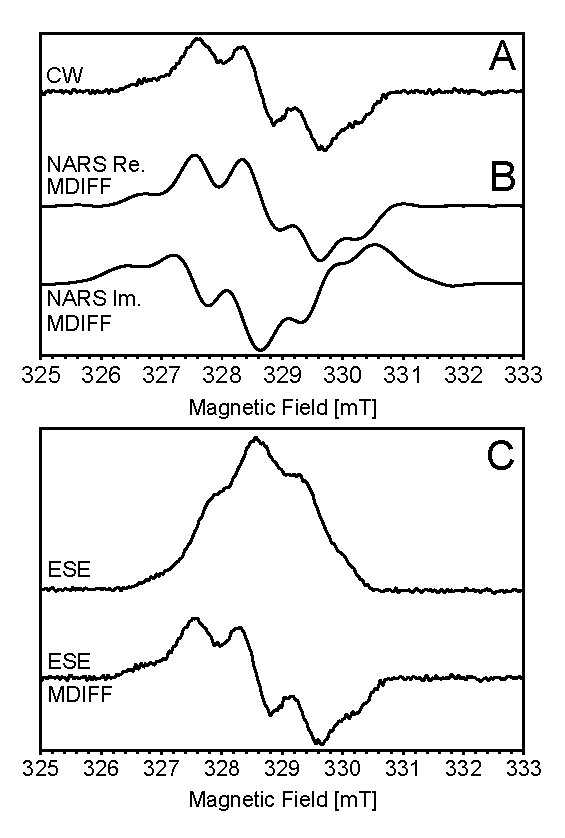
\includegraphics{Kapitel/Ch4-Images/02-PSII-BBY-Data.eps}
\caption[Frozen solution EPR on a 85~nl volume sample at X-band.]{Frozen solution EPR on a 85~nl volume sample at X-band Three EPR experiments performed with a 0.4~mm inner diameter self-resonant micro-helix. Shown are the A) continuous-wave, B) real and imaginary non-adiabatic rapid scan (NARS), and C) field-swept two-pulse electron spin-echo (ESE) EPR experiments of the tyrosine D radical (Y$_D^\bullet$) in photosystem II with 85~nl of frozen solution sample at a temperature of 80~K. Calculated moving difference (MDIFF) pseudo-modulation of 0.5~mT is shown for the NARS and field-swept ESE experiments in order to directly compare to the continuous-wave EPR experiment. The total time for the experiments were 49, 55, and 45 minutes, respectively. The signal-to-noise ratio is calculated and tabulated in Table~\ref{table:snrcalc}.}
\label{fig:BBYPSII}
\end{figure}

Shown in Fig.~\ref{fig:BBYPSII} is the Y$_D^\bullet$ radical EPR signal in an 85~nl frozen solution from photosystem II (BBY particles) at a temperature of 80~K using the self-resonant micro-helix. A continuous-wave EPR experiment, shown in Fig.~\ref{fig:BBYPSII}A, was performed an Elexsys E580 X-band bridge by sweeping 10~mT in 1 minute (4096 points) with a modulation rate of 100~kHz and an amplitude of 0.5~mT. The data was averaged 49 times for a total of 49 minutes at an incident power of 0.2~$\mu$W. To further improve the signal-to-noise ratio of the continuous-wave experiment, a field-swept non-adiabatic rapid scan (NARS) experiment was performed, data shown in Fig.~\ref{fig:BBYPSII}B. The field-swept non-adiabatic rapid scan (NARS) experiment was performed on the same commercial hardware using the rapid-scan method of M\"{o}ser {\em et al.}\cite{MOSER2017} and processed with the method described in Hyde {\em et al.}\cite{Hyde2013MDIFF} Herein, the scan rate was a sinusoidal 100~kHz field-sweep at 1~mT amplitude and a field-step size of 0.05~mT. The collected real and imaginary, pure-absorption and pure-dispersion, spectra were pseudo-modulated with a 0.5~mT moving difference (MDIFF)\cite{Hyde2013MDIFF} to compare to the field-modulated continuous-wave experiment. A factor of 2 in signal-to-noise improvement is obtained for the same signal acquisition time. 

A field-swept two-pulse electron spin-echo (ESE) EPR experiment was performed on the same commercial hardware over a 8~mT sweep, shown in Fig.~\ref{fig:BBYPSII}C. The field-swept ESE data was pseudo-modulated with a 0.5~mT MDIFF to compare the experiment with the field-modulated continuous-wave experiment of Fig.~\ref{fig:BBYPSII}A. The signal-to-noise ratio for all three experiments were calculated and tabulated in Table~\ref{table:snrcalc}. 

\begin{table}[htbp]
\centering
\caption[Signal-to-noise calculations.]{Signal-to-noise calculations for the three experiments performed on the photosystem II Y$_D^\bullet$ radical in frozen solution at a temperature of 80~K. Approximately 1.6$\times10^{12}$ spins were calculated to be in the 85~nl that fill the micro-helix.}
\begin{tabular}{llll}
\multicolumn{1}{l|}{Experiment} & \multicolumn{1}{l|}{SNR Re.} & \multicolumn{1}{l|}{SNR Im.} & Time\\ \hline\hline
\multicolumn{1}{l|}{Continuous Wave} & \multicolumn{1}{c|}{197} & \multicolumn{1}{c|}{131} & \multicolumn{1}{c}{49~min} \\\hline
\multicolumn{1}{l|}{NARS} & \multicolumn{1}{c|}{4400} & \multicolumn{1}{c|}{2300} & \multicolumn{1}{c}{55~min} \\\hline
\multicolumn{1}{l|}{NARS (MDIFF)} & \multicolumn{1}{c|}{410} & \multicolumn{1}{c|}{423} & \multicolumn{1}{c}{--} \\\hline
\multicolumn{1}{l|}{ESE} & \multicolumn{1}{c|}{248} & \multicolumn{1}{c|}{--} & \multicolumn{1}{c}{45~min} \\\hline
\multicolumn{1}{l|}{ESE (MDIFF)} & \multicolumn{1}{c|}{106} & \multicolumn{1}{c|}{--} & \multicolumn{1}{c}{--}\\
\end{tabular}\label{table:snrcalc}
\end{table}

\begin{figure}[htbp]
\centering
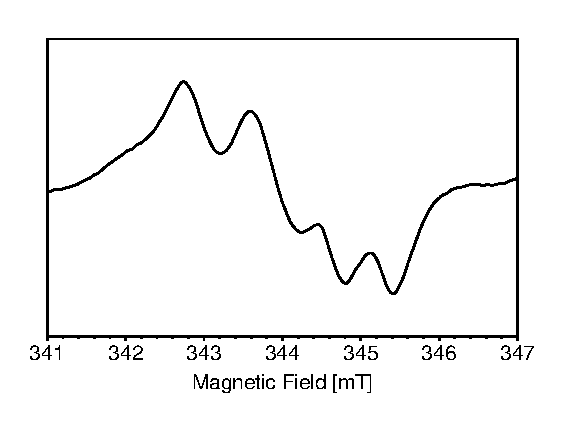
\includegraphics{Kapitel/Appendix/Images/S5-BBYMD5.eps}
\caption[CW EPR of frozen solution photosystem II in the Bruker MD5W1.]{Continuous-wave EPR of frozen solution photosystem II sample performed in the Bruker MD5W1 dielectric resonator at a temperature of 80~K. A signal-to-noise ratio of approximately 300 is calculated for 636~nl of sample.}
\label{fig:BBYMD5}
\end{figure}

Finally, a comparison between the MD5W1 dielectric resonator and the self-resonant micro-helix was performed with the frozen solution photosystem II (BBY particle) sample at a temperature of 80~K. A continuous-wave EPR experiment was performed to compare the EPR signal obtained with 85~nl volume in the micro-helix. The photosystem II sample was placed in a 0.3~mm inner diameter quartz tube with a sample height of 9~mm (636~nl) and centered in the dielectric cavity. A signal-to-noise ratio of approximately 300 is calculated for the 636~nl of sample, shown in Fig.~\ref{fig:BBYMD5}. The spectrum was collected by sweeping 10~mT in 1 minute (4096 points) with a modulation rate of 100~kHz and an amplitude of 0.5~mT. The data are averaged 49 times for a total time of 49 minutes at an incident power of 3.1~$\mu$W. This power was chosen to compare the two samples at approximately the same microwave magnetic field incident on the sample. Normalizing the signal-to-noise ratio with the volume yields a factor of approximately 5 improvement of absolute spin sensitivity using the self-resonant micro-helix compared to the MD5W1. These experiments serve to show the versatility of the micro-helix to perform EPR experiments on limited sample volumes (less than 85~nl) at X-band.

\paragraph{Single-Crystal continuous-wave EPR of the tyrosine D radical (Y$_D^\bullet$) in photosystem II core complex.}
Shown in Fig.~\ref{fig:xTalPSII} is continuous-wave EPR data collected at two separate angles of the photosystem II Y$_D^\bullet$ radical in a single crystal at a temperature of 80~K as a sensitivity test for the 0.4~mm inner diameter self-resonant micro-helix. The photosystem II core complex crystal had a volume of 0.3 $\times$ 0.18 $\times$ 0.18~mm$^3$. The spectra were collected by sweeping 15~mT in 1 minute (4096 points) with a modulation rate of 100~kHz and an amplitude of 0.3~mT. The data are averaged 49 times for a total time of 49 minutes at an incident power of 0.2~$\mu$W. Simulations using the known $g$-tensor and hyperfine tensors \cite{Hofbauer6623} were performed with an Easyspin (http://easyspin.org, Ref.~[5.\kern-0.4em\citenum{STOLL200642}]; reproduced in Appendix~C) global fit routine to find the crystal orientation and plotted in red in Fig.~\ref{fig:xTalPSII}. At X-band, the g-anisotropy of the Y$_D^\bullet$ radical is very small and is not resolved. Instead, the orientation dependence is primarily determined by the hyperfine interaction pattern of the coupled proton nuclei. \cite{Hofbauer6623} Using only two angles, a unique fit cannot be found, but a demonstration of the Y$_D^\bullet$ features is shown. A non-specifically bound Mn$^{2+}$ signal is also present in the crystal, yielding the signals indicated by an asterisk (\mbox{\large $\ast$}). 

\begin{figure}[htbp]
\centering
 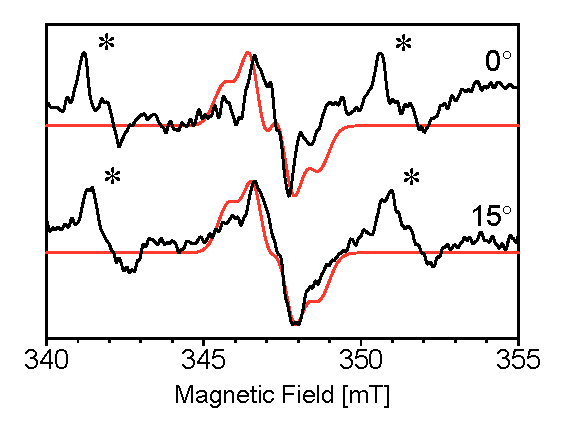
\includegraphics{Kapitel/Ch4-Images/03-PSII-xTal-Data.eps}
 \caption[Single-Crystal CW EPR of Y$_D^\bullet$ in photosystem II core complex.]{Single-Crystal continuous-wave EPR of Y$_D^\bullet$ in photosystem II core complex. Continuous-wave EPR collected with the 0.4~mm inner diameter self-resonant micro-helix at two angles of the photosystem II Y$_D^\bullet$ radical from a single crystal at a temperature of 80~K. The crystal size was 0.3 $\times$ 0.18 $\times$ 0.18~mm$^3$. Shown in red is a fitted simulation with similar features. A non-specifically bound Mn$^{2+}$ signal is also present in the mother-liquor of the crystal, indicated by an asterisk (\mbox{\large $\ast$}). Each spectrum was collected in 49 minutes with a signal-to-noise ratio of approximately 35.}
 \label{fig:xTalPSII}
\end{figure}

The use of photosystem II crystals as a benchmark provides a challenging system to measure. The photosystem II core complex has a molecular weight of approximately 455~kDa as a monomer and each complex contains only one Y$_D^\bullet$ radical. With a crystal size of 0.3 $\times$ 0.18 $\times$ 0.18~mm$^3$, a known average size of the unit cell, and that there are 8 photosystem II complexes per unit cell, one can calculate approximately 8.9$\times10^{12}$ Y$_D^\bullet$ radicals to be present in the sample. This demonstrates the versatility of the micro-helix to study large complexes in small crystal dimensions. A photosystem II core complex crystal can be routinely grown to dimensions of 0.3~mm, but requires significant effort to increase in size. Finally, the Y$_D^\bullet$ radical is easily saturable with large microwave magnetic fields, which limits the available microwave power and maximum EPR signal at a given temperature. Despite these challenges, a signal-to-noise of approximately 35 is calculated for the Y$_D^\bullet$ radical. 

\section{Conclusions and Outlook}
An application of the self-resonant micro-helix geometry and planar-coupling structure that increases the EPR absolute spin sensitivity by a factor of approximately 28 if the signal is unsaturable and 6 if the EPR signal is able to be saturated is presented. For saturable EPR signals, such as those found in protein samples, the self-resonant micro-helix saves up to a factor of 32 in measuring time. From this gain in sensitivity, the self-resonant micro-helix is well-suited for EPR studies on protein single-crystals with dimensions less than 0.3~mm. Due to the very high efficiency parameter of 3.2~mT/W$^{1/2}$, which corresponds to a $\pi/2$ pulse of 20~ns with an incident power of 20~mW, the micro-helix geometry is advantageous in extending pulse EPR to experiments that usually require costly high-powered microwave amplifiers (e.g. HYSCORE), further expanding the applicability of pulse EPR. We also show that the micro-helix performs well for field-swept non-adiabatic rapid scan (NARS) techniques due to its small size and ``open'' structure, which increases the continuous-wave EPR spin sensitivity further by a factor of 2 for the same experimental time. Due to the relatively large bandwidth of the micro-helix (90~MHz critically-coupled), this geometry is particularly well-suited for frequency-swept NARS and rapid scan experiments which further improve the signal-to-noise ratio for saturable samples\cite{Hyde2013MDIFF, MOSER2017} and for the use of arbitrary-waveform generators for advanced pulse spectroscopy. \cite{schweiger2001principles, chirpedESEEM, goldfarb2018epr}

The micro-helix Q-value and high efficiency parameter $\Lambda_{ave}$ of make the resonator suitable for watching the onset of the EPR signal during pulses. This resonator may allow us to approach ``dead-time free'' EPR for FID excitation. For example, if we assume a typical pulse X-band bandwidth of 70~MHz and a $Q_0$-value of 1000, a $\beta$ of 6.5 is needed to over-couple the cavity to the desired bandwidth. If we also assume it takes 15 time constants (factor of 2 for voltage detection) for the ring-down of the cavity 
\begin{equation}
    15 \time \tau_c = 15 \times 2 \times Q / 2 \pi \nu
\end{equation}
where $\nu$ is the frequency of interest. This produces a dead-time of 67~ns. For the micro-helix, with a critically-coupled measured $Q_0$-value of 220 the dead-time is 55~ns. (While critically-coupled, the signal-to-noise is improved by a $\sqrt{2}$ compared to an over-coupled cavity.) If we assume we can over-couple the micro-helix by a $\beta$ of 6.5, this leads to a dead-time of 15~ns. However, compared to the Bruker MS3, the micro-helix would need a factor of 10 less power for the same B$_1$, lowering the number of time constants needed.

As this technology matures, further improvements to enhance the sensitivity based on new fabrication techniques and choice of other materials will be explored. Not only does the increase in sensitivity save time in EPR data measurements, but also reduces the need of the availability of, or necessity to, grow larger crystals. Overall, the self-resonant micro-helix provides the possibility to study catalytically-active proteins at crystal dimensions relevant to X-ray crystallography and, as such, is a significant advancement in the field of enzyme research. 

{\renewcommand{\bibsection}{\clearpage\section*{\bibname}\markboth{\bibname}{\bibname}}
\renewcommand{\bibname}{CHAPTER 5. REFERENCES}
\bibliographystyle{elsarticle-num}
\bibliography{Kapitel/Ch5-References}
}
